\documentclass[12pt]{article}

\usepackage[utf8x]{inputenc}
\usepackage[L7x, T2A]{fontenc}
\usepackage[lithuanian]{babel}
\usepackage{vwcol}  
\usepackage{sectsty}
\usepackage{setspace}
\usepackage{fancyhdr}
\usepackage{graphicx}
\usepackage{ragged2e}
\usepackage{titlesec}
\usepackage{epsfig}
\usepackage{indentfirst}
\usepackage[top=2cm, bottom=2cm, left=3cm, right=1.5cm]{geometry}

\usepackage{svg}

\makeatletter
\expandafter\let\csname L7x-cmd\endcsname\@changed@cmd
\makeatother

\addto\extraspolish{\fontencoding{L7x}\selectfont}
\addto\noextraspolish{\fontencoding{\encodingdefault}\selectfont}

\setlength\parindent{1cm}

\title{VILNIAUS UNIVERSITETAS \bigbreak \bigbreak 
MATEMATIKOS IR INFORMATIKOS FAKULTETAS \bigbreak \bigbreak 
PROGRAMŲ SISTEMŲ KATEDRA}
\author{}
\date{}

\pagestyle{fancy}
\fancyhead{}
\fancyfoot{}
\fancyfoot[R]{\thepage}
\renewcommand{\headrulewidth}{0pt}

%\renewcommand{\thesection}{}

\begin{document}
	\clearpage
	\maketitle
	\thispagestyle{empty}

	\begin{center}
		\begin{Large}
			\textbf{Transporto priemonių skelbimų aplikacija} \bigbreak
		\end{Large}
		\begin{large}
			\textbf{Application for Vehicle Advertisement} \bigbreak
		\end{large}
		Programų sistemų inžinerijos I laboratorinis darbas Nr. 1 \bigbreak

		\bigbreak
		\bigbreak
		\bigbreak
		\bigbreak
		\bigbreak
		\bigbreak
		\bigbreak

		\begin{tabular}{ll}
			Atliko:        & 2 kurso 5 grupės studentai \\
		               	   & Toma Burneikaitė \\
		               	   & Žygimantas Stongvilas \\
		                   & Mantas Jurčius \\
		                   & Rimvydas Meškauskas \\
			Darbo vadovas: & asist., dr., Vytautas Valaitis
		\end{tabular}

		\bigbreak
		\bigbreak
		\bigbreak
		\bigbreak
		\bigbreak
		\bigbreak
		\bigbreak
		\bigbreak
		\bigbreak
		\bigbreak
		\bigbreak
		\bigbreak
		\bigbreak
		\bigbreak
		\bigbreak

		Vilnius - 2018
	\end{center}
	\pagebreak
	
	\section*{Anotacija}
	\addcontentsline{toc}{section}{Anotacija}
	\begin{indent}
	Šiame projektiniame darbe pristatomas automobilių skelbimų programėlės „AutoInf“ įgyvendinimas. Projektas „AutoInf“ skirta  palengvinti automobilio paieškas internete. Programėlė, skirta mobiliesiems įrenginiams, suteikia galimybę vartotojui legviau rasti jį dominančią transporto priemonę, sujungdama visus skelbimus, esančius Europos automobilių pardavimo skelbimų puslapiuose. Programų sistemos architektūra apibrėžiama naudojantis 4+1 architektūros pjūvių modelį. Toliau pristatomi programos reikalavimai, bei pateikiama dalykinės srities analizė.
	\end{indent}
	\pagebreak

	\tableofcontents
	\pagebreak

	\section*{Įvadas}
	\addcontentsline{toc}{section}{Įvadas}
	
	\begin{flushleft}
		\bigbreak\textbf{Programų sistemos pavadinimas}
	\end{flushleft}
	
	Pilnas programų sistemos pavadinimas – automobilių skelbimų aplikacija „AutoInf“ \\
	
	\begin{flushleft}
		\textbf{Dalykinė sritis}
	\end{flushleft}	
	
	Automobilių skelbimų iš visos Europos pateiktis vartotojams  \\
	
	\begin{flushleft}
		\textbf{Probleminė sritis}
	\end{flushleft}
	
	Užsienyje galima rasti pigesnių automobilių \\
	
	\begin{flushleft}
		\textbf{Naudotojai} 
	\end{flushleft}
	
	Žmonės, ieškantys automobilių \\
	
	\begin{flushleft}
		\textbf{Darbo pagrindas}
	\end{flushleft}
	
	Dokumentas parengtas kaip programų sistemos inžinerijos dalyko laboratorinis darbas\\Nr. 1, kuriame pateikiamas suprojektuotos sistemos aprašymas.
	\pagebreak

	\section{Projektavimas}
	\subsection{Užduotys ir jų vykdymo scenarijai}
	\subsubsection{Sistemos vykdomos užduotys}
	Žemiau pavaizduotoje diagramoje pavaizduoti tikslai, kurių siekia sistema besinaudojantys agentai - automobilių ieškantys vartotojai bei sistemos administratoriai. Į sistemą žiūrima kaip į vieną visumą, neatskleidžiant jos implementacijos detalių.
	
	\begin{figure}[h]
		\begin{center}
			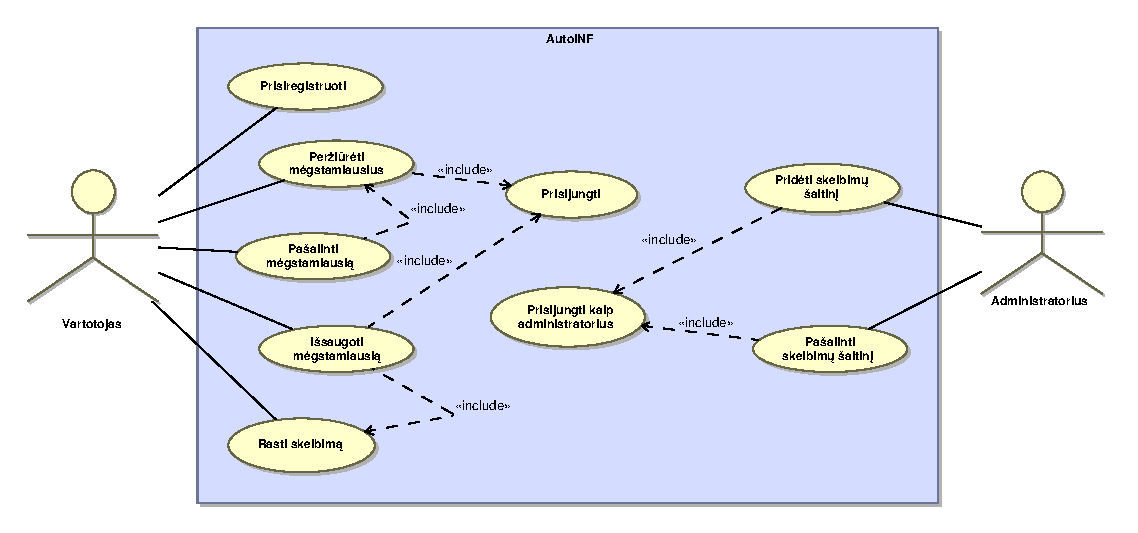
\includegraphics[width=\textwidth]{Tikslai.eps}
			\caption{Sistemos užduočių diagrama\label{UseCase}}
		\end{center}
	\end{figure}
	
	Diagramoje \ref{UseCase} yra pavaizduoti tikslai, kurių siekia sistema besinaudojantys agentai - vartotojas ir administratorius
	\pagebreak

	\begin{figure}[h]
		\begin{center}
			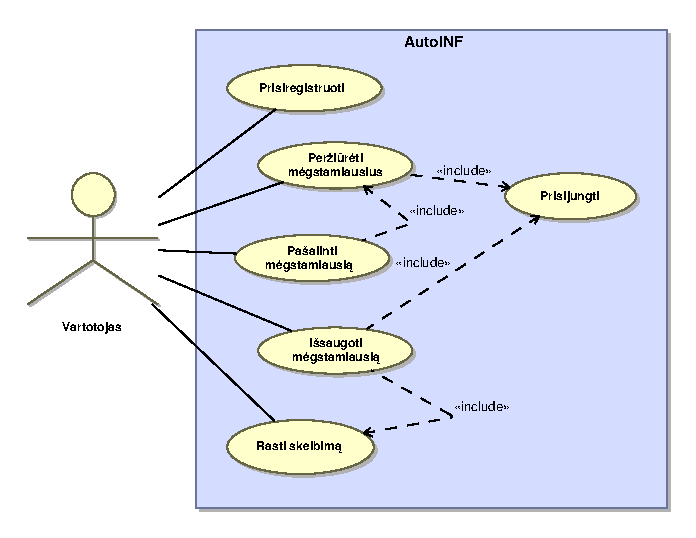
\includegraphics[width=0.7\textwidth]{TikslaiVartotojas.eps}
			\caption{Sistemos užduočių diagrama iš vartotojo perspektyvos\label{UseCaseUser}}
		\end{center}
	\end{figure}
	
	Diagramoje \ref{UseCaseUser} pateiktos vartotojui prieinamos „AutoINF“ funkcijos: registracija, prisijungimas, peržiūrėti mėgstamiausius, pašalinti mėgstamiausius, išsaugoti mėgstamiausius, rasti skelbimą. Plačiau apie šias funkcijas rašoma tolimesnėse sekų diagramose.
	\pagebreak	
	
	\begin{figure}[h]
		\begin{center}
			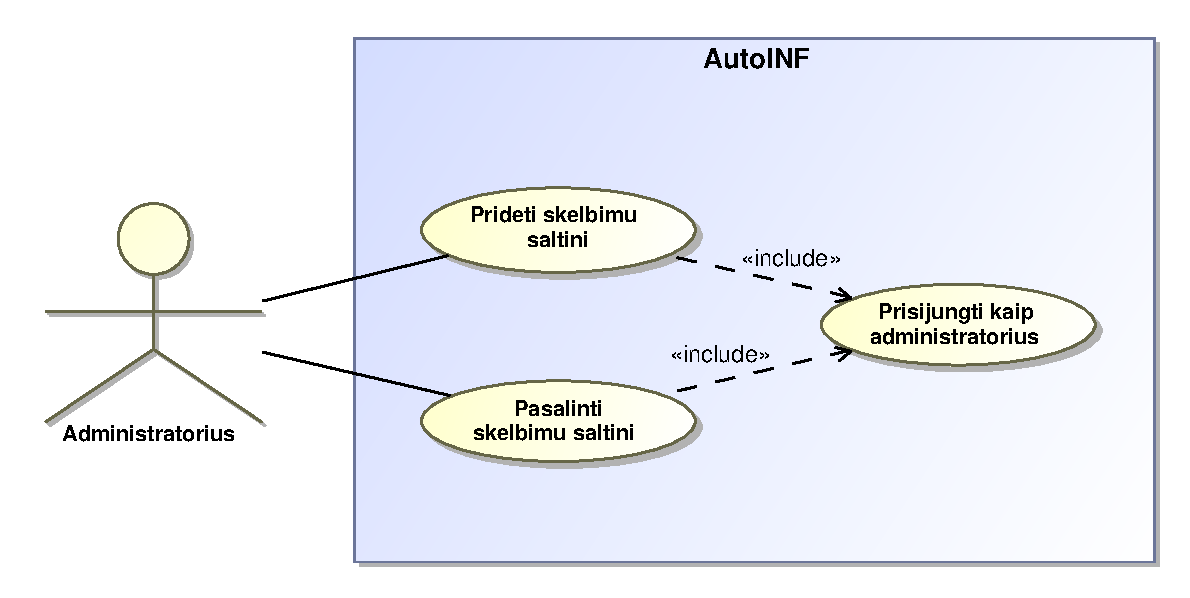
\includegraphics[width=0.7\textwidth]{TikslaiAdministratorius.eps}
			\caption{Sistemos užduočių diagrama iš administratoriaus perspektyvos\label{UseCaseAdmin}}
		\end{center}
	\end{figure}	
	
	Diagramoje \ref{UseCaseAdmin} pateiktos administratoriui prieinamos „AutoINF“ funkcijos: pridėti skelbimų šaltinį, pašalinti skelbimų šaltinį, pašalinti vartotojo paskyrą. Plačiau apie šias funkcijas rašoma tolimesnėse sekų diagramose. Administratorius prisijungia taip pat kaip ir vartotojas, tik jam suteiktos administratoriaus teisės.
	\pagebreak
	
	\subsubsection{Užduoties „Prisiregistruoti“ įgyvendinimas}
	
	\begin{figure}[h]
		\begin{center}
			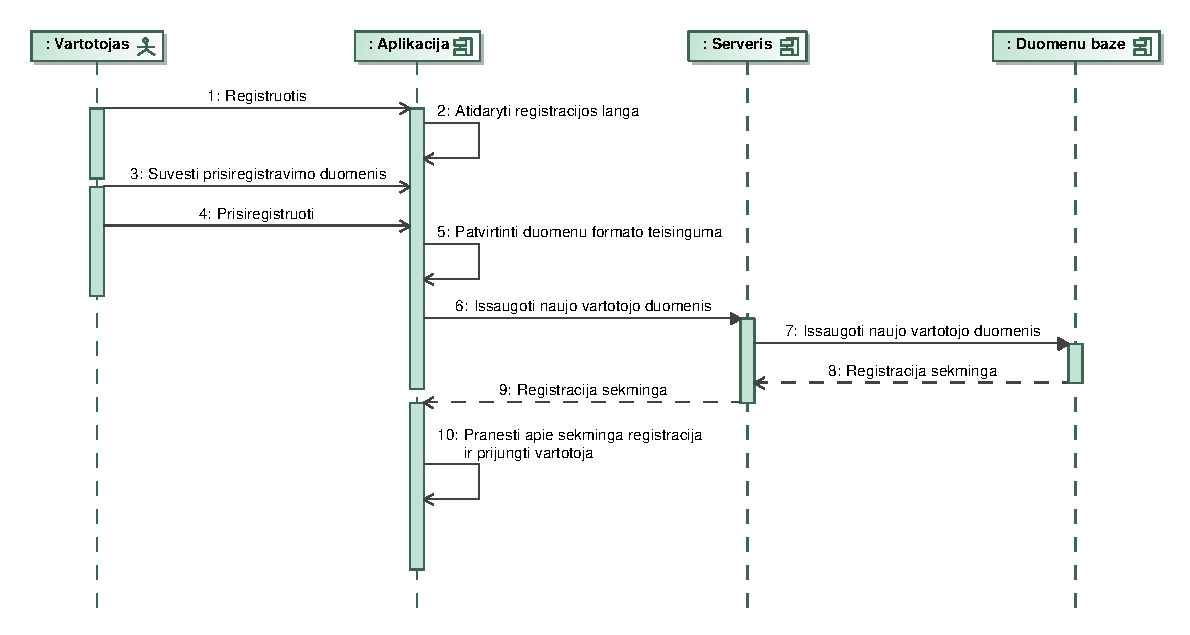
\includegraphics[width=\textwidth]{Prisiregistruoti.eps}
			\caption{Užduoties „Prisiregistruoti“ sekų diagrama\label{RegisterSeq}}
		\end{center}
	\end{figure}
	
	\ref{RegisterSeq} diagramoje pavaizduotas vartotojo registracijos sistemoje užduoties vykdymas. Vartotojas, atidaręs registracijos langą, turi suvesti prisiregistravimo duomenis. Paspaudus registracijos mygtuką, aplikacija patikrina, ar duomenys suvesti reikiamu formatu. Jei formatas teisingas, tai duomenys išsaugomi duomenų bazėje. Tada vartotojas yra infomuojamas apie sėkmingą registraciją ir yra prijungiamas prie sistemos.
	\pagebreak
	
	\subsubsection{Užduoties „Prisijungti“ įgyvendinimas}
	
	\begin{figure}[h]
		\begin{center}
			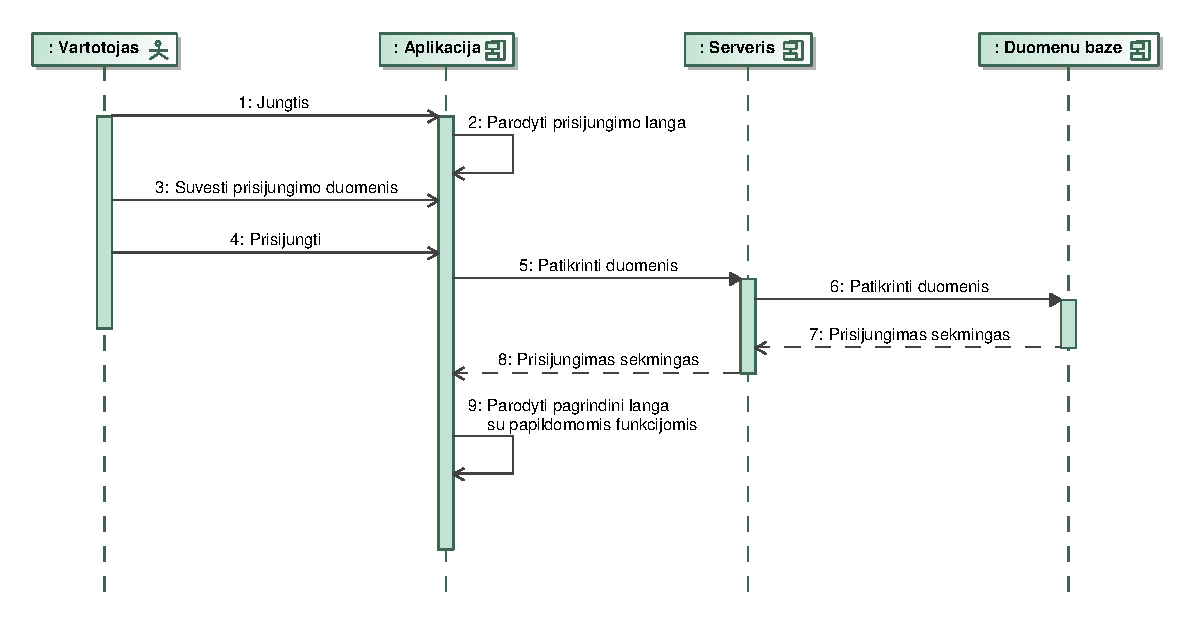
\includegraphics[width=\textwidth]{Prisijungti.eps}
			\caption{Užduoties „Prisijungti“ sekų diagrama\label{LogInSeq}}
		\end{center}
	\end{figure}
	
	\ref{LogInSeq} diagramoje pavaizduotas vartotojo prisijungimo sistemoje užduoties vykdymas. Vartotojas, atidaręs prisijungimo langą, turi suvesti prisijungimo duomenis ir tada paspaudus prisijungimo mygtuką, duomenų bazėje yra patikrinama, ar toks vartotojas egzistuoja. Vartotojui prisijungus atsidaro pagrindinis langas, kuriame atsiranda funkcijos, prieinamos tik registruotiems vartotojams.
	\pagebreak
	
	\subsubsection{Užduoties „Rasti skelbimą“ įgyvendinimas}
	
	\begin{figure}[h]
		\begin{center}
			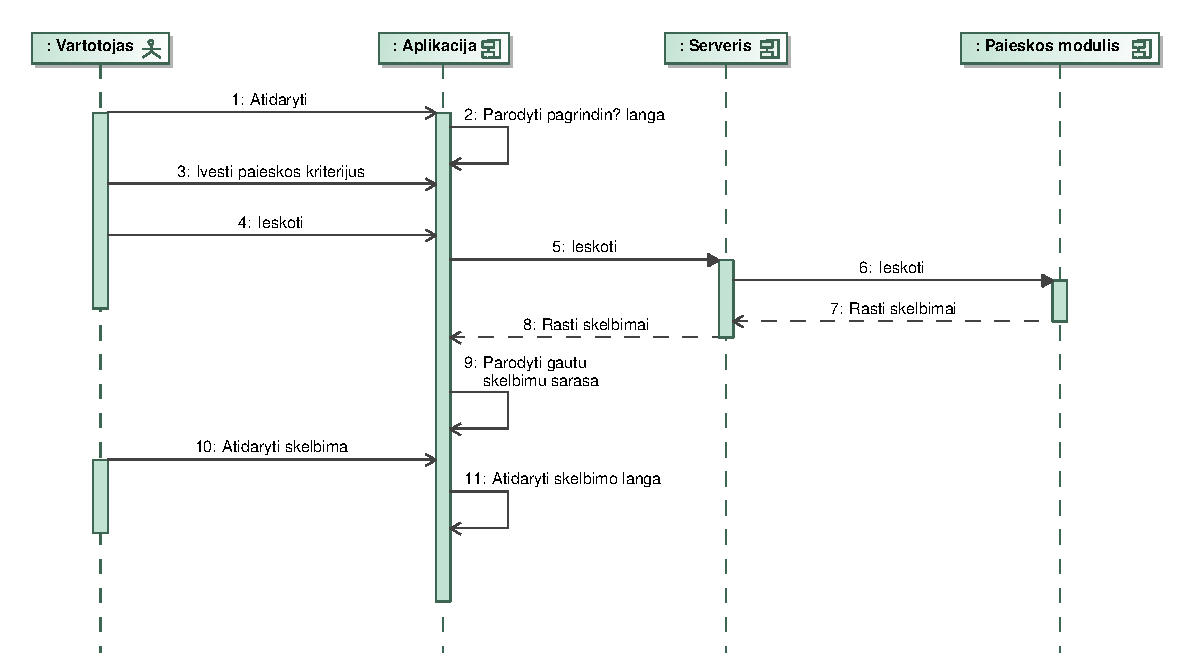
\includegraphics[width=\textwidth]{RastiSkelbima.eps}
			\caption{Užduoties „Rasti skelbimą“ sekų diagrama\label{FindAdvertSeq}}
		\end{center}
	\end{figure}
	
	\ref{FindAdvertSeq} diagramoje pavaizduotas skelbimų ieškojimo sistemoje užduoties vykdymas. Vartotojas nebūtinai turi būti prisijungęs, norint naudotis šia sistemos funkcija. Pirmiausia vartotojas turi pagrindiniame lange įvesti paieškos kriterijus (kai kurie filtrai yra privalomi). Paspaudus paieškos mygtuką, sistema suranda filtrą atitinkančius skelbimus ir parodo juos. Vartotojui paspaudus ant skelbimo atsidaro skelbimo langas.
	\pagebreak
	
	\subsubsection{Užduoties „Išsaugoti mėgstamiausią“ įgyvendinimas}
	
	\begin{figure}[h]
		\begin{center}
			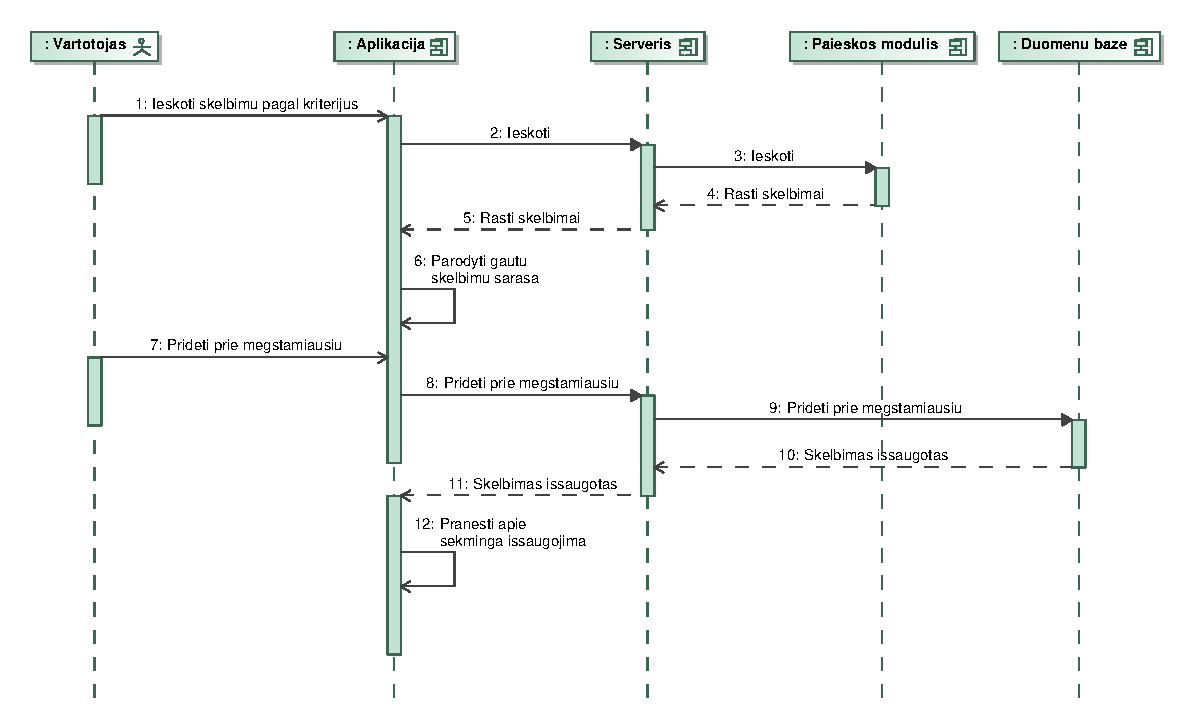
\includegraphics[width=\textwidth]{IssaugotiMegstamiausia.eps}
			\caption{Užduoties „Išsaugoti mėgstamiausią“ sekų diagrama\label{SaveFavSeq}}
		\end{center}
	\end{figure}
	
	\ref{SaveFavSeq} diagramoje pavaizduotas mėgstamiausio skelbimo išsaugojimo užduoties vykdymas. Ši funkcija yra pasiekiama tada ir tik tada, kai vartotojas yra prisijungęs prie sistemos. Norint išsaugotį skelbimą, vartotojas pirmiausiai turi susirasti skelbimą, ir tada prie jo paspausti skelbimo išsaugojimo mygtuką. Apie sėkmingą skelbimo išsaugojimą vartotojas yra informuojamas.
	\pagebreak
	
	\subsubsection{Užduoties „Pašalinti mėgstamiausią“ įgyvendinimas}
	
	\begin{figure}[h]
		\begin{center}
			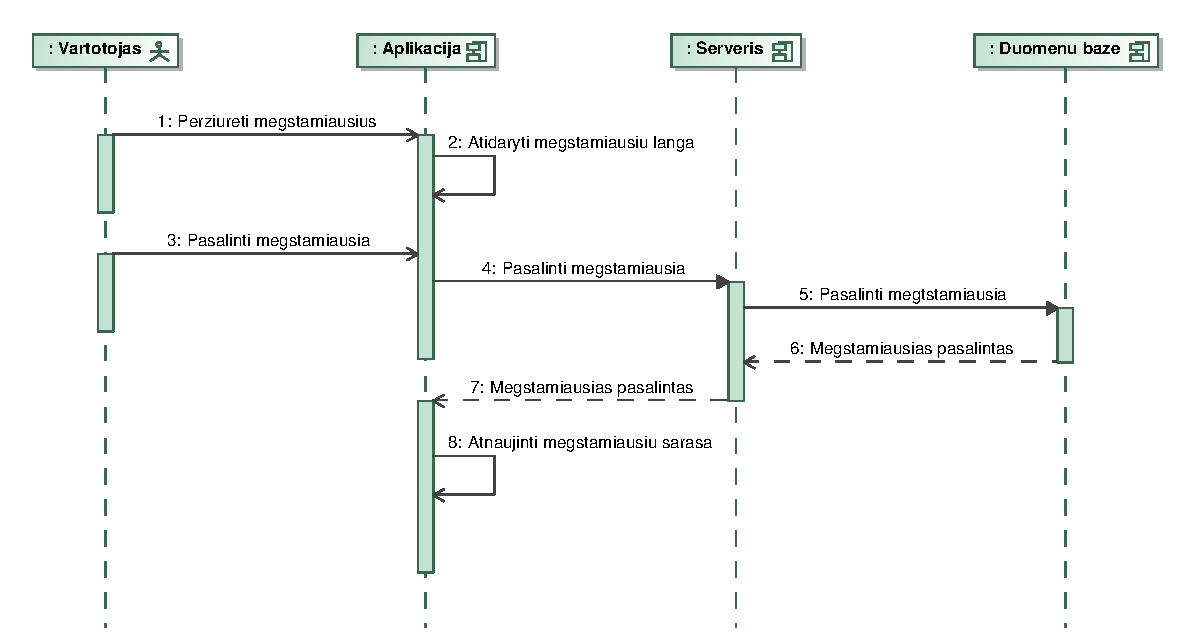
\includegraphics[width=\textwidth]{PasalintiMegstamiausia.eps}
			\caption{Užduoties „Pašalinti mėgstamiausią“ sekų diagrama\label{DelFavSeq}}
		\end{center}
	\end{figure}
	
	\ref{DelFavSeq} diagramoje pavaizduotas mėgstamiausio skelbimo pašalinimo užduoties vykdymas. Ši funkcija yra pasiekiama tada ir tik tada, kai vartotojas yra prisijungęs prie sistemos. Pirmiausiai vartotojas atsidaro mėgstamiausių skelbimų sąrašą. Pasirenką kurį skelbimą jis nori pašalinti ir paspaudus pašalinimo mygtuką. Sėkmingai pašalinus skelbimą iš sąrašo, šis sąrašas yra atnaujinamas.
	\pagebreak
	
	\subsubsection{Užduoties „Peržiūrėti mėgstamiausius“ įgyvendinimas}
	
	\begin{figure}[h]
		\begin{center}
			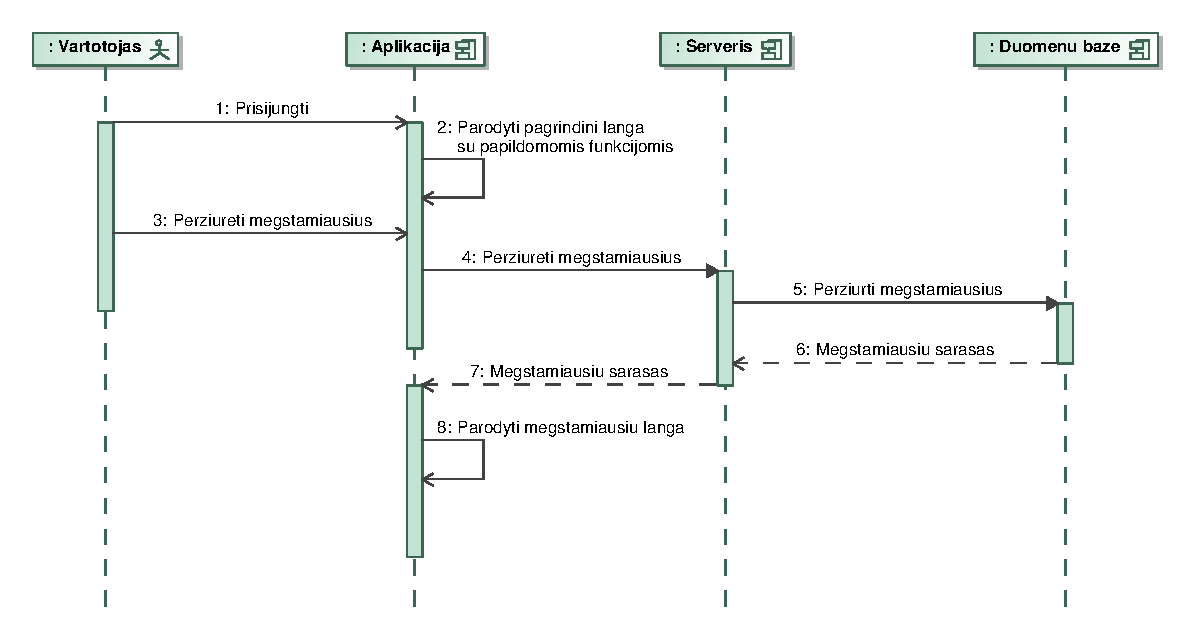
\includegraphics[width=\textwidth]{PerziuretiMegstamiausius.eps}
			\caption{Užduoties „Peržiūrėti mėgstamiausius“ sekų diagrama\label{ViewFavSeq}}
		\end{center}
	\end{figure}
	
	\ref{ViewFavSeq} diagramoje pavaizduotas peržiūrėti mėgstamiausius skelbimus užduoties vykdymas. Ši funkcijas pasiekiama tada ir tik tada, kai vartotojas yra prisijungęs prie sistemos. Vartotojui pasirinkus mėgstamiausių skelbimų langą, sistema parodo šio vartotojo mėgstamiausių skelbimų sarašą.
	\pagebreak
	
	\subsubsection{Užduoties „Tvarkyti skelbimų šaltinius“ įgyvendinimas}
	
	\begin{figure}[h]
		\begin{center}
			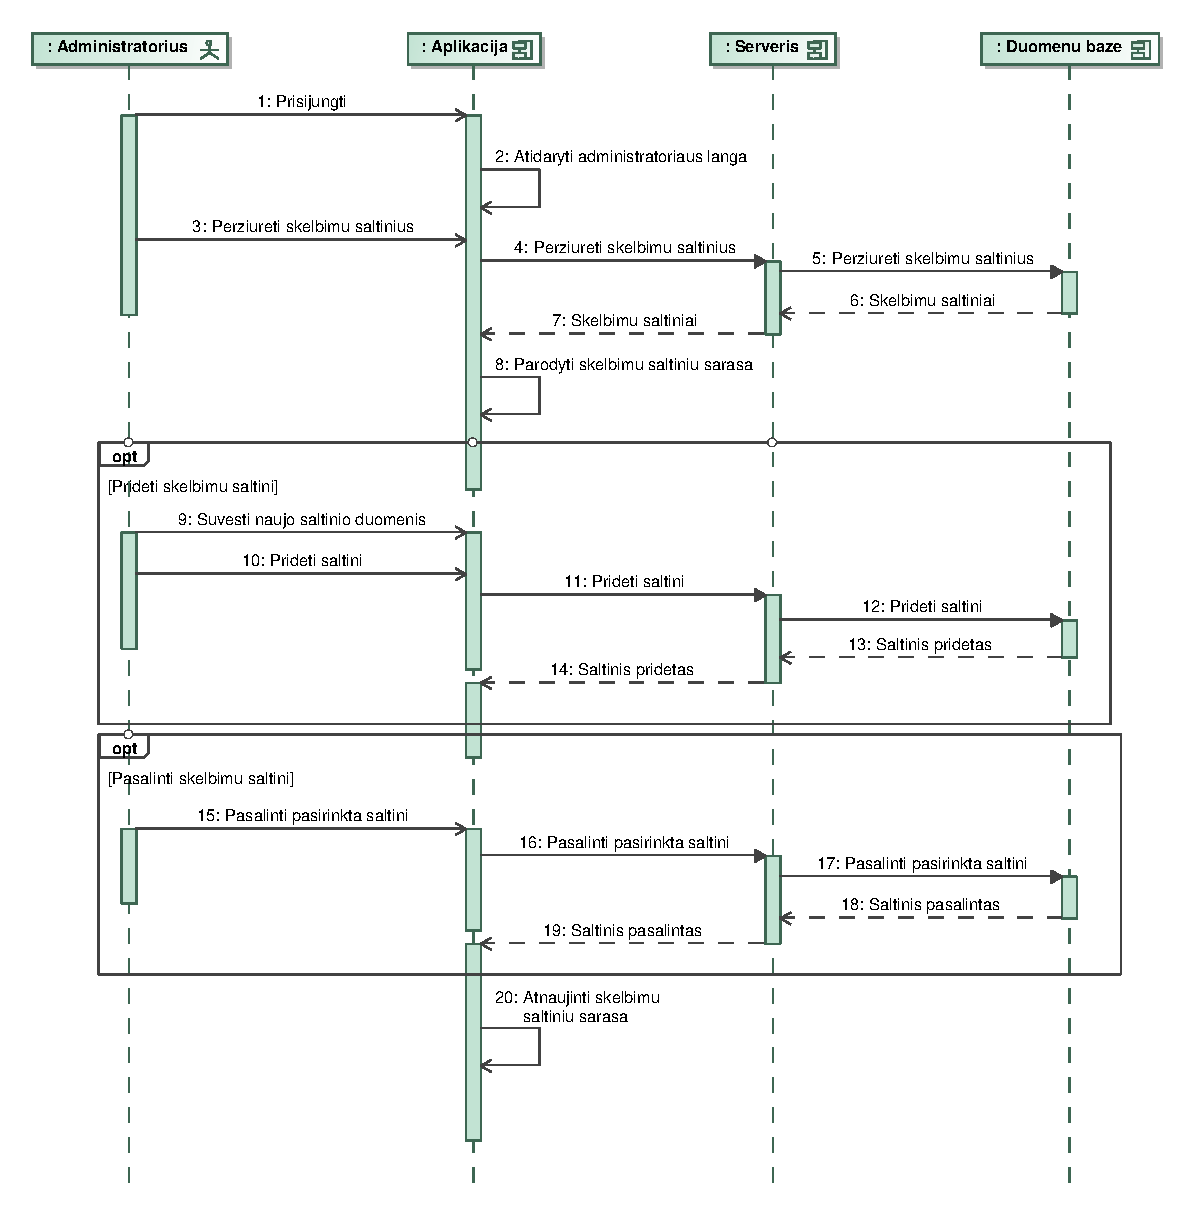
\includegraphics[width=0.8\textwidth]{TvarkytiSkelbimuSaltinius.eps}
			\caption{Užduoties „Tvarkyti skelbimų šaltinius“ sekų diagrama\label{ManSouSeq}}
		\end{center}
	\end{figure}
	
	\ref{ManSouSeq} diagramoje yra pavaizduotas skelbimų šaltinių tvarkymo užduoties vykdymas. Šia funkcija gali pasinaudoti tik administratorius. Administratorius atsidaręs skalbimų šaltinių langą gali pasirinkti, ką jis nori su šaltiniais daryti: pridėti naują skelbimų šaltinį arba pašalinti šaltinį. Norint pridėti šaltinį, administratorius spaudžia mygtuką skirtą naujam šaltiniui pridėti, o norint pašalinti skelbimą, administratorius turi pasirinkti šaltinį iš šaltinių sąrašo, ir pasirinkti šaltinio pašalinimą. Tiek po šaltinio pridėjimo, tiek po šaltinio pašalinimo, skelbimų šaltinių sąrašas yra atnaujinamas.
	\pagebreak
	
	\subsection{Struktūrinis programų sistemos modelis}
	\subsubsection{Klasių diagrama}
	
	Žemiau pateiktoje klasių diagramoje yra išskirtos pagrindinės esybės, kurios yra naudojamos sistemoje. Klases siejantys ryšiai pasižymi kardinalumu. Kitaip sakant, nustatytas konkretus ryšių skaičius ar skaičių aibė, kurios turės klasės egzempliorius su tam tikros kitos klasės egzemplioriais.
	
	\begin{figure}[h]
		\begin{center}
			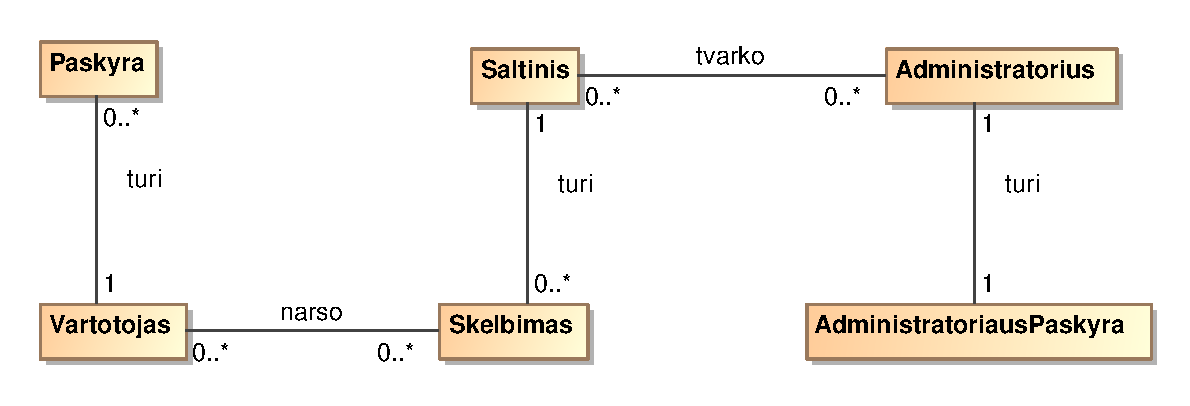
\includegraphics[width=\textwidth]{KlasiuDiagrama.eps}
			\caption{Užduoties „Klasių diagrama“ sekų diagrama\label{ClassDiagram}}
		\end{center}
	\end{figure}
	
	Šioje sistemoje egzistuoja dviejų rūšių paskyros: paprasta paskyra, ir administratoriaus paskyra. Paprastas vartotojas gali turėti daug paskyrų(pvz.: pamiršta visus duomenis apie savo paskyrą, tai jis gali susikurti naują), o paskyra priklauso tik vienam vartotojui. Administratorius gali turėti tik vieną paskyrą, vartotojui išduodamas vienkartinis kodas, kurį įvedus sukuriama specialią administratoriaus paskyrą. Administratorius tvarko šaltinius(t.y. prideda arba pašalina šaltinius). Kiekvienas šaltinis gali būti tvarkomas kelių arministratorių, ir taip pat kiekvienas administratorius gali tvarkyti kelis šaltinius. Vartotojai gali naršyti daug skelbimų ir visi kelbimai gali būti naršomi kelių vartotojų. Visi skelbimai yra paimti iš kokių nors šaltinių. Kiekvienas skelbimas gali būti paimtas tik iš vieno šaltinio, tačiau visi šaltiniai gali turėti daug skelbimų.
	\pagebreak
	
	\subsubsection{Objektų diagrama}
	
	Šiame skyrelyje esančios objektų diagramos iš esmės patvirtina anksčiau pateiktą klasių diagramą. Taip pat pateikia tipinių pavyzdžių, kaip klasės bus naudojamos sistemoje.
	
	\begin{figure}[h]
		\begin{center}
			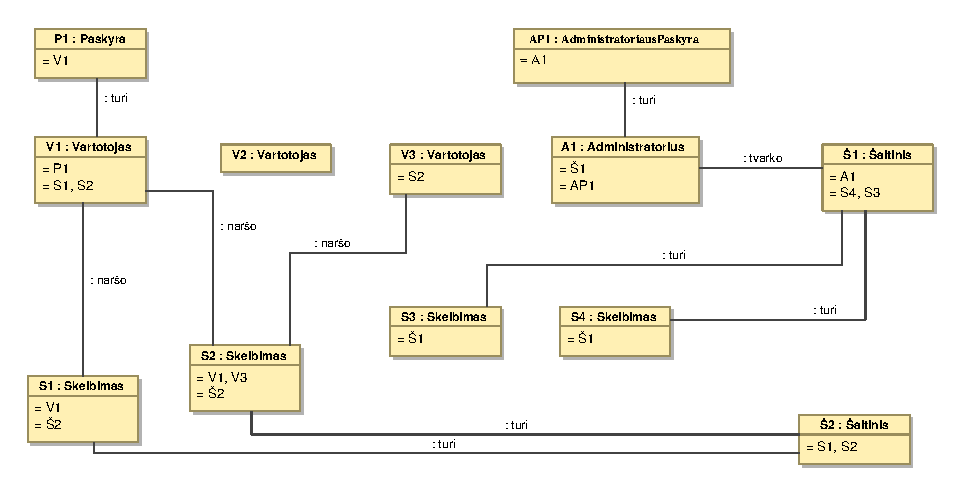
\includegraphics[width=\textwidth]{ObjektuDiagrama.eps}
			\caption{Užduoties „Objektų diagrama“ sekų diagrama\label{ObjectDiagram}}
		\end{center}
	\end{figure}
	
	\ref{ObjectDiagram} diagramoje parodyta tipinė sistemos situacija, kai yra sukurtos dvi paskyros, viena yra vartotojo, kita administratoriaus. Taip pat yra dar du vartotojai, vienas iš jų tuo momentu nieko nedaro sistemoje, kol kitas, kartu su registruotu vartotoju, naršo skelbimus (keli vartotojai gali naršyti tą patį skelbimą vienu metu). Taip pat yra keturi skelbimai, ir visi priklauso kažkuriam vienam šaltiniui, kol šaltiniai turi daugiau nei po vieną skelbimą (šaltiniai gali ir neturėti skelbimų). Taip pat iš diagramos galima matyti, kad administratorius gali tvarkyti šaltinius.
	\pagebreak
	
	\subsection{Programų sistemos komponentai}
	
	Sistemos komponentų dekompozicija įgyvendinta "top-down" būdu.	
	
	\subsubsection{Konteksto diagrama}
	
	\begin{figure}[h]
		\begin{center}
			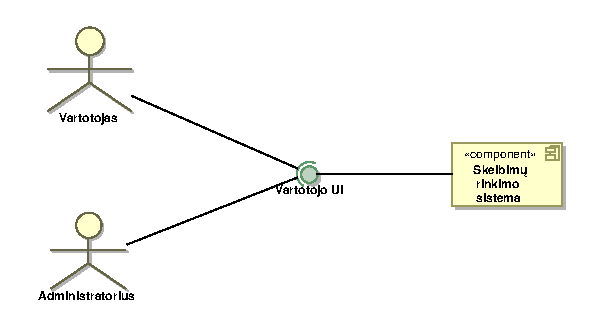
\includegraphics[width=\textwidth]{Komponentai1.eps}
			\caption{Konteksto komponentų diagrama\label{Components1}}
		\end{center}
	\end{figure}
	
	\ref{Components1} diagramoje prodomas abstrakčiausias (aukščiausias) komponentų struktūros lygis. Visa sistema laikoma kaip vienas darinys, ir parodoma sąsaja su išore:
	
	\begin{itemize}	
		\item Interfeisai, kuriais išoriniai vartotojai naudojasi visa sistema
		\item Išorinių sistemų interfesiai, kuriais naudojasi sistema
	\end{itemize}
	
	Tiek vartotojas, tiek administratorius turi naudotis tuo pačiu vartotojo UI interfeisu. To priežastis yra tai, kad abu vartotojai naudojasi ta pačia sistema, tik su šiek tiek skirtingomis galimybėmis.	
	\pagebreak

	\subsubsection{Skelbimų rinkimo sistemos dekompozicija}

	\begin{figure}[h]
		\begin{center}
			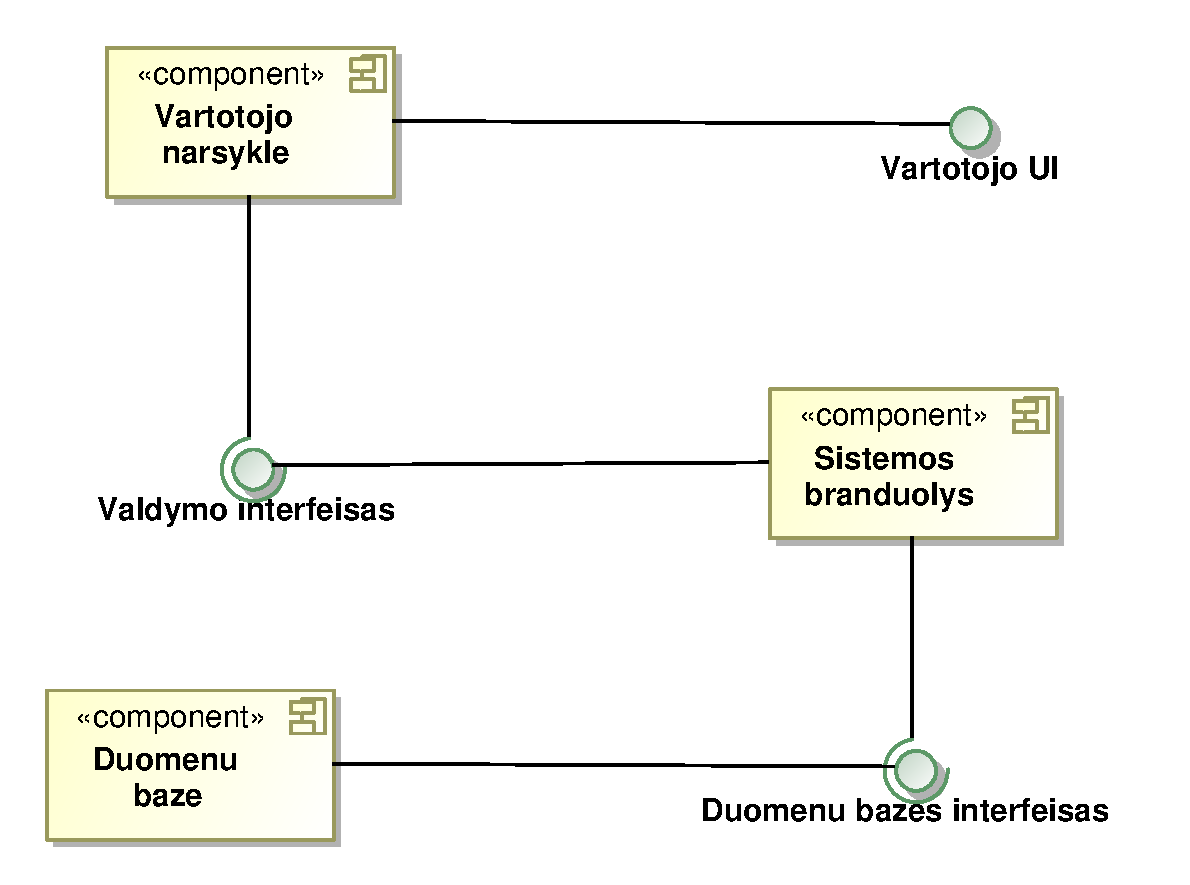
\includegraphics[width=\textwidth]{Komponentai2.eps}
			\caption{Skelbimų rinkimo sistemos komponento dekompozicija\label{Components2}}
		\end{center}
	\end{figure}
	
	\ref{Components2} diagramoje detalizuojamas \ref{Components1} diagramoje esantis „Skelbimų rinkimo sistema“\\

	\textbf{Vartotojo naršyklė} - komponentas, sukuriantis vartotojo interfeisą bei vykdantis komunikaciją tarp vartotojo ir sistemos branduolio.\\

	
	\textbf{Sistemos branduolys} - komponentas, priimantis prašymus iš vartotojo naršyklės, kontroliuojantis duomenų gavimą ar išsaugojimą duomenų bazėje bei siunčiantis duomenis vartotojo naršyklei.\\

	
	\textbf{Duomenų bazė} - komponentas, kuriame saugoma informacija apie registruotus vartotojus ir kartu tos paskyros mėgstamiausius skelbimus.\\
	\pagebreak

	\subsubsection{Sistemos branduolio dekompozicija}
	
	\begin{figure}[h]
		\begin{center}
			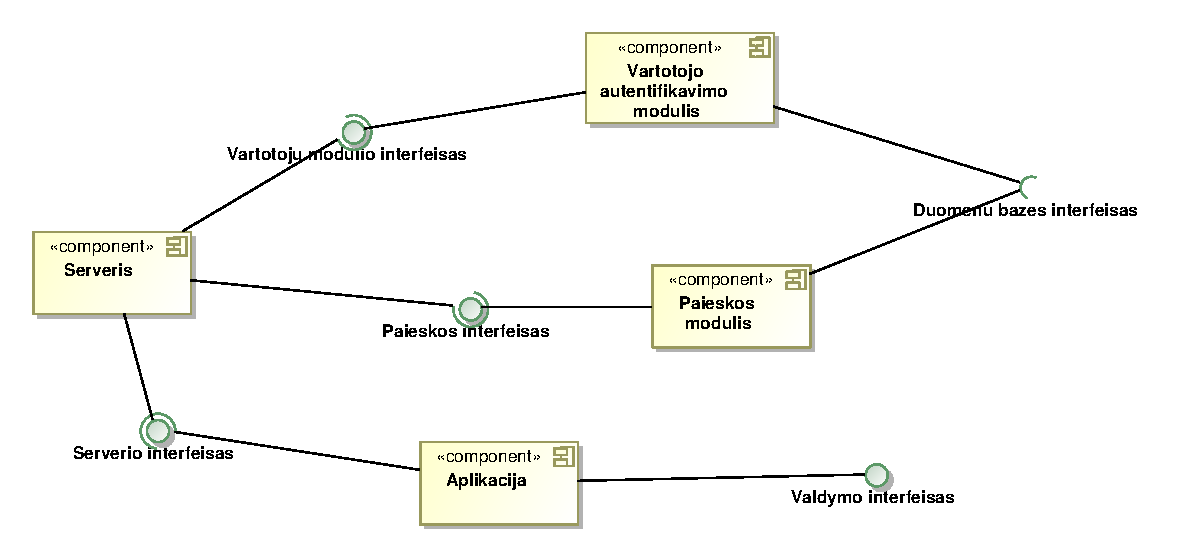
\includegraphics[width=\textwidth]{Komponentai3.eps}
			\caption{Sistemos branduolio komponento dekompozicija\label{Components3}}
		\end{center}
	\end{figure}

	\ref{Components3} diagramoje smulkinamas \ref{Components2} diagramoje esantis „Sistemos branduolio“ komponentas. Jį sudarantys komponentai:\\
	
	\textbf{Vartotojo autentifikavimo modulis} - šis komponentas vykdo vartotojų autetifikaciją. Jo funkcijos: vartotojų registravimas, prisijungimas.\\
	
	\textbf{Paieškos modulis} - pagal tam tikrus nurodytus kriterijus suranda skelbimus.\\
	
	\textbf{Serveris} - komponentas, valdantis prieigą prie duomenų.\\
	
	\textbf{Aplikacija} - komponentas, kuris pateikia vartotojui skelbimų sąrašą, konkrečių skelbimų detlesnę informaciją.
	\pagebreak

	\subsection{Dinaminis programų sistemos modelis}
	\subsubsection{Veiklos diagrama}
	
	\begin{figure}[h]
		\begin{center}
			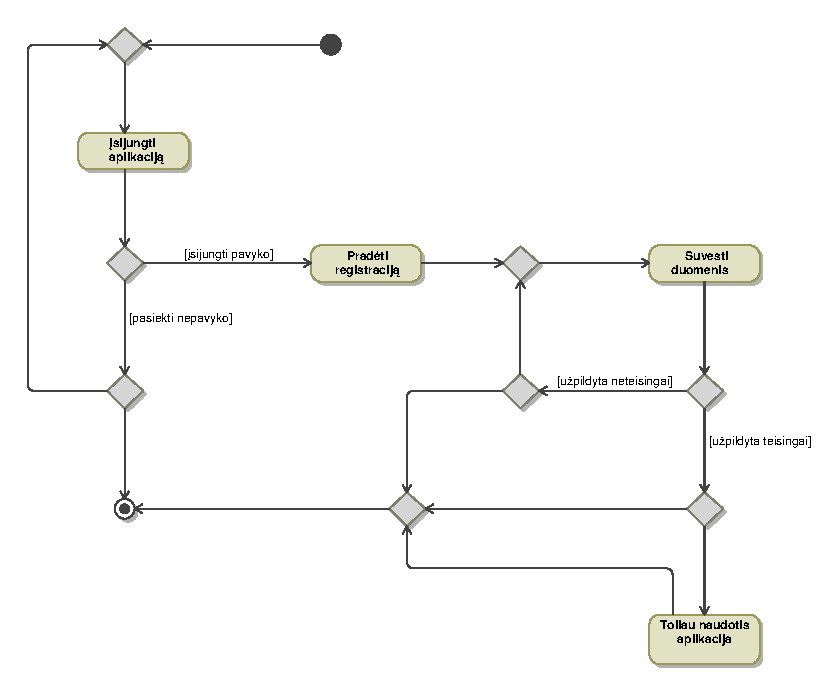
\includegraphics[width=\textwidth]{RegistracijosVeikla.eps}
			\caption{Vartotojo registracijos veiklos diagrama\label{RegisterActivity}}
		\end{center}
	\end{figure}
	
	\ref{RegisterActivity} diagramoje parodyti procesai vykstantys registracijos metu. Registravimas vyksta tada, kai vartotojas įsijungia aplikaciją ir pasirenka „Registraciją“. Tada, vartotojui suvedus reikiamus duomenis, sistema patikrina, ar viskas užpildyta teisingai, jei ne, tai vartotojas gali bandyti vesti informaciją iš naujo, arba išeitį iš registravimosi lango. Jei informacija užpildyta teisingai, tai vartotojas gali toliau naudotis aplikacija, arba išeiti iš jos.
	\pagebreak
	
	\begin{figure}[h]
		\begin{center}
			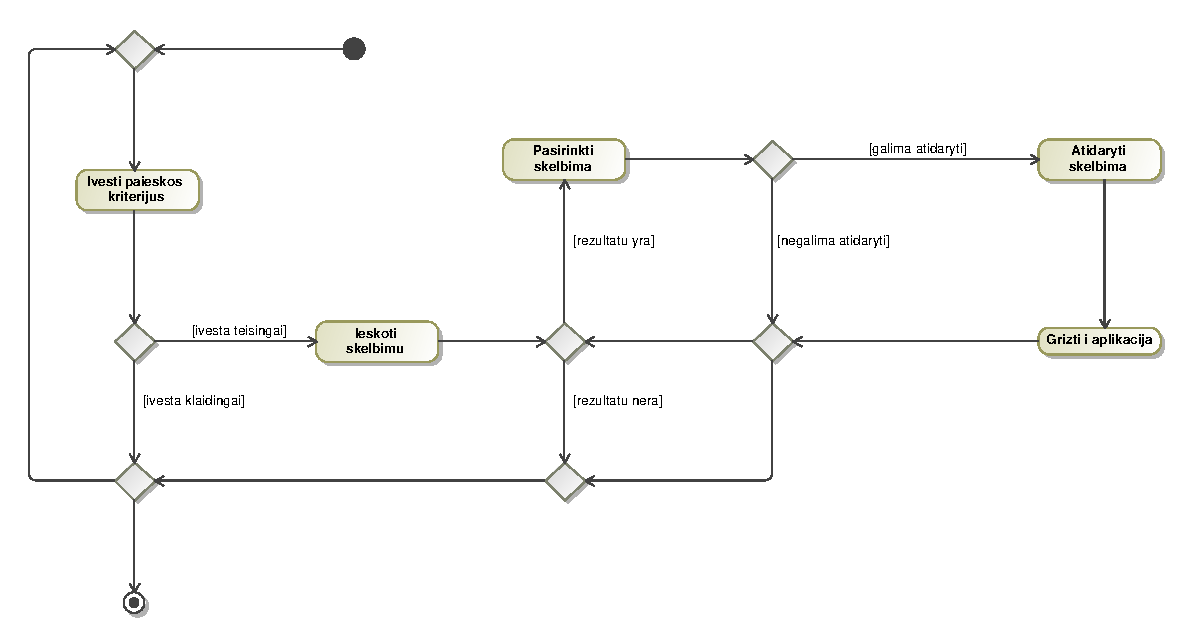
\includegraphics[width=\textwidth]{PaieskosVeikla.eps}
			\caption{Skelbimų paieškos veiklos diagrama\label{SearchActivity}}
		\end{center}
	\end{figure}
	
	\ref{SearchActivity} diagramoje parodyti procesai vykstantys skelbimo ieškojimo metu. Pagrindiniame lange vartotojas turi įvesti filtrus, pagal kuriuos bus ieškomi skelbimai. Sistema patikrina, ar įvesti kriterijai yra teisingai suvesti. Jei įvesta klaidingai, tai vartotojai gali bandyti iš naujo suvesti paieškos kriterijus, arba išeiti iš programos. Jei paieškos kriterijai įvesti teisingai, tai sistema ieško skelbimų, jei rezultatų nėra, tai galima pasirinkti kitokius filtruas arba išeiti iš programos. Suradus rezultatų, vartotojas gali pasirinkti skelbimą, jei jo negalima atidaryti galima bandyti paiešką atlikti iš naujo, jei galima atidaryti, tai vartotojas gali atidaryti skelbimą ir po to grįžti į aplikaciją.
	\pagebreak

	\begin{figure}[h]
		\begin{center}
			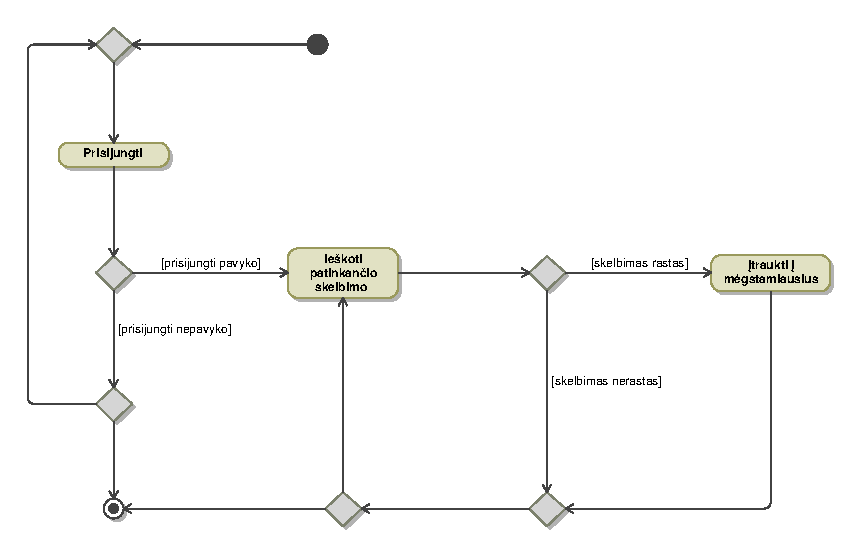
\includegraphics[width=\textwidth]{MegstamiausiuVeikla.eps}
			\caption{Naujo mėgstamiausio skelbimo veiklos diagrama\label{FavActivity}}
		\end{center}
	\end{figure}
	
	\ref{FavActivity} diagramoje parodyti procesai vykstantys vartotojui norint įtraukti skelbimą į mėgstamiausių sąrašą. Pirmiausia vartotojas turi prisijungti, jei to padaryti nepavyksta, jis gali bandyti iš naujo arba išeiti iš programos. Prisijungus prie sistemos, vartotojas ieško jam patinkantį skelbimą, suradus jį, vartotojas galį įtraukti į mėgstamiausiųjų sąrašą, o po to ieškoti naujo skelbimo, arba išeiti iš šito lango. Jei patinkančio skelbimo vartotojas neranda, tai gali bandyti ieškoti iš naujo arba išeiti iš šito lango.
	\pagebreak
	
	\subsection{Komponentų išskirstymas tinkle}
	\subsubsection{Komponentų ryšių su artifaktais diagrama}
	
	\ref{ArtComp} pateiktoje komponentų ryšių su artifaktais diagramoje su artifaktais yra išskirti pagrindiniai sistemos artifaktai. Artifaktus ir komponentus tarpusavyje sieja manifestacijos ryšys. Tai reiškia, kad artifakto sudaromoji dalis yra konkretus komponentas.
	
	\begin{figure}[h]
		\begin{center}
			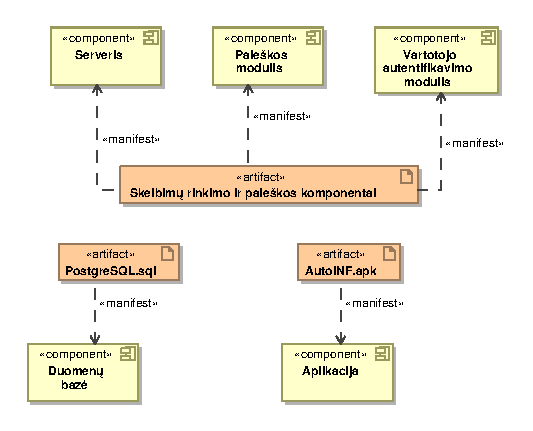
\includegraphics[width=0.8\textwidth]{ArtifaktaiKomponentai.eps}
			\caption{Komponentų ryšių su artifaktais diagrama\label{ArtComp}}
		\end{center}
	\end{figure}

	Sistema susidaro iš triejų pagrindinių dalių - aplikacijos, skelbimų rinkimo ir paieškos komponentų ir duomenų bazės. Informacijai saugoti apie vartotojų paskyras pasirinkta PostgreSQL duomenų bazė.
	\pagebreak
	
	\subsubsection{Mazgų diagrama}
	
	Žemiau pateiktoje mazgų diagramoje yra išskirti fiziniai įrenginiai, rekalingi sistemos darbo palaikymui bei artifaktų pasiskirstymas tarp jų.\\
	
	\begin{figure}[h]
		\begin{center}
			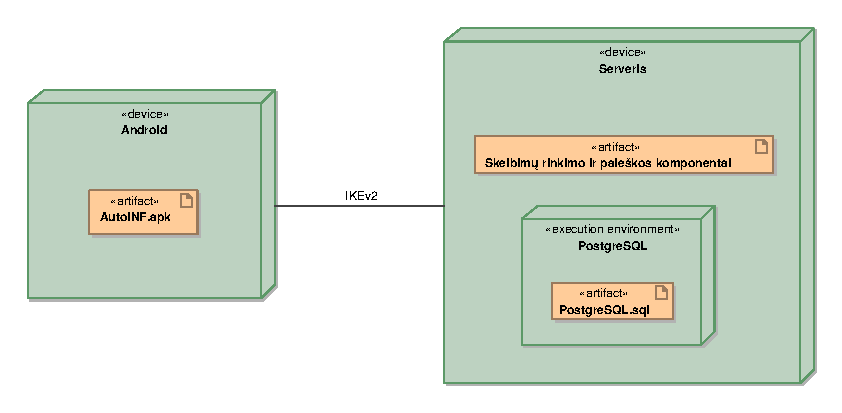
\includegraphics[width=0.9\textwidth]{Mazgai.eps}
			\caption{Mazgų diagrama\label{Cube}}
		\end{center}
	\end{figure}
	
	Visa sistema yra laikoma serveryje. Šiame serveryje yra sudiegiami skelbimų rinkimo ir paieškos komponentai. Tame pačiame serveryje yra ir PostgreSQL duomenų bazė. Vartotojui, norint naudotis sistema iš mobiliojo įrenginio, siunčiama užklausa IKEv2 protokolu siekiant gauti sistemos failus.
	\pagebreak
	
	
	\section*{Išvada}
	\addcontentsline{toc}{section}{Išvada}
	Šiame laboratoriniame darbe pasitelkiant skirtingus sistemos pjūvius aprašyta knygų dalinimosisistemos architektūra. Užduočių pjūvyje išsiaiškinti pagrindiniai agentų tikslai naudojantis sistema. Loginis pjūvis leido išskirti pagrindines esybes bei ryšius tarp jų. Kūrimo pjūvyje atlikta sistemos dekompozicija pradedant nuo bendro komponento toliau jį detalizuojant.Procesų pjūvyje išskirti procesai, jų komunikacija, objektų gyvavimo ciklai. Galiausiai fiziniame pjūvyje apibrėžtas sistemos išdėstymas tinkle. Šis skirtingų požiūrių rinkinys leido iš anksto aptikti sistemoje galimas klaidas bei sukurti tinkamą sistemos architektūrą.
	\pagebreak

	\section*{Terminų žodynas}
	\addcontentsline{toc}{section}{Terminų žodynas}	
	
	\bigskip
	\textbf{Vartotojas} - žmogus, besinaudojantis sistema.\\
	
	\textbf{Skelbimas} - iš šaltinio gautas skelbimas.\\
	
	\textbf{Šaltinis} - puslapis, iš kurio gaunami skelbimai.\\
	\pagebreak

	\section*{Literatūros sąrašas}
	\addcontentsline{toc}{section}{Literatūros sąrašas}	
	
	Doug Rosenberg and Matt Stephens “Use Case Driven Object Modeling with UML“
\end{document}